\documentclass{standalone}
\usepackage{tikz}
\usepackage{pgfplots}
\pgfplotsset{compat=1.18}
\usetikzlibrary{arrows.meta}

\begin{document}

\resizebox{8cm}{8cm}{%
    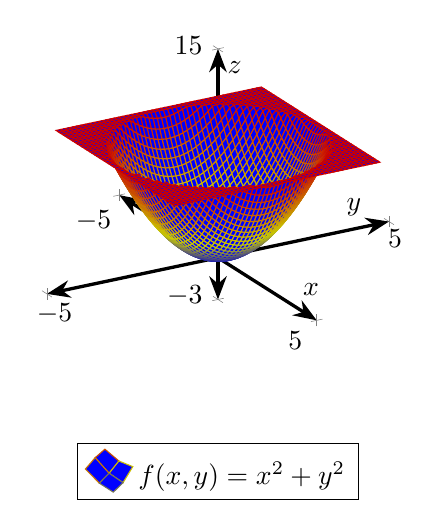
\begin{tikzpicture}
    \begin{axis}[
        % title={3D Surface: $z = x^2 + y^2$},
        axis lines=middle,
        axis line style={Stealth-Stealth,very thick},
        xlabel={$x$},
        ylabel={$y$},
        zlabel={$z$},
        xmin=-5,xmax=5,ymin=-5,ymax=5, zmin=-3, zmax=15,
        xtick distance=1,
        ytick distance=1,
        ztick distance=2,
        grid=major,
        grid style={thin,densely dotted,black!20},
        view={60}{30}, % Adjust the viewing angle
        % Numbers on axes
        xtick={-5, 5},
        ytick={-5, 5},
        ztick={-3, 0, 5, 8, 15},
        % colormap/viridis,
        % colorbar,
        % colorbar style={
        %    title={$z$},
        % Legend
        legend style={
            at={(0.5,-0.1)}, % Position at the center bottom
            anchor=north, % Anchor the legend at the top
            cells={anchor=west} % Align the legend entries to the left
        }
    ]
    % Plot the function
    \addplot3[
        surf,
        domain=-3:3,
        domain y=-3:3,
        samples=50,
        color=blue,
    ]
    {min(x^2 + y^2, 8)}; % z capped at 8

    \addlegendentry{$f(x, y) = x^2 + y^2$}

    \end{axis}
    \end{tikzpicture}
}

\end{document}